Fyrr í bókinni höfum við farið yfir fjórar grunnaðgerðir sem nauðsynlegar eru til gagnagrunnsvinnslu. Við kunnum að
\begin{itemize}
 \item Búa til gagnagrunna og töflur (\verb|CREATE| skipanir, kaflar \ref{undirkafli:synidaemi-i-sql} og \ref{undirkafli:bua-til-toflu})
 \item Setja gögn inn í töflur (\verb|INSERT| skipunin, \ref{undirkafli:innsetning})
 \item Ná í gögn úr töflum (\verb|SELECT| skipunin, kaflar \ref{kafli:select} og \ref{kafli:gagnavinnslamargartoflur} eins og þeir leggja sig)
 \item Eyða töflum og öllu sem í þeim er (\verb|DROP| skipunin, kafli \ref{undirkafli:drop})
\end{itemize}
Þetta kemur okkur býsna langt. Þetta hefur hins vegar ekki leyft okkur að gera nokkrar breytingar á töflum eða þeim gögnum sem í þeim eru. Til þess þurfum við fleiri skipanir. Þær heita \verb|ALTER TABLE|, \verb|UPDATE| og \verb|DELETE|.
\section{DDL og DML}
\begin{marginfigure}[-6cm]
\caption[DDL og DML]{Yfirlit yfir þær SQL-skipanir sem við höfum séð og flokkun þeirra í DDL og DML.}
\label{mynd:ddl-dml}
\centering
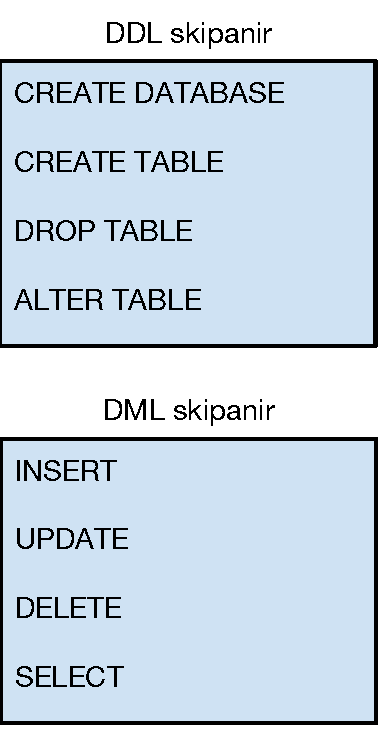
\includegraphics[width=\linewidth]{myndir/ddl-dml}
\end{marginfigure}
Áður en lengra er haldið skulum við staldra við og skoða þær skipanir sem við höfum þegar kynnst.

Þessar skipanir, \verb|CREATE|, \verb|INSERT|, \verb|SELECT| og \verb|DROP| skiptast í tvo flokka. Flokkarnir kallast \emph{Data Definition Language} (DDL) og \emph{Data Manipulation Language} (DML).\footnote{Þessir flokkar hafa verið kallaðir \emph{gagnaskilgreiningarmál} og \emph{gagnameðferðarmál} á íslensku.}

DDL skipanir hafa áhrif á uppbyggingu gagnagrunnsins. Þær breyta, búa til og eyða gagnagrunnum, töflum og dálkum. \verb|CREATE| skipanir og \verb|DROP| skipunin eru DDL skipanir.

DML skipanir hafa áhrif á gögn í gagnagrunninum. Þær breyta, búa til, eyða og sýna innihald taflna. \verb|INSERT| og \verb|SELECT| eru DML skipanir.\footnote{\emph{SELECT} skipunin er örlítið sérstök hvað DML skipanir varðar, þar sem hún hefur það ekki að aðalhlutverki að breyta gögnum. Þess vegna er oft fjallað um hana sérstaklega. Hún er DML skipun engu að síður.}

Fleiri flokkar skipana eru til. Þær skipanir sem við förum yfir í þessari bók falla þó allar í þessa tvo.
\section{Að breyta töflum}
Hingað til höfum við ekki farið yfir leið til að breyta töflum. Það þýðir að í hvert skipti sem villa er gerð í töflu höfum við þurft að henda töflunni ásamt öllu því sem í henni er (\verb|DROP TABLE|) og búa hana til upp á nýtt.

Þetta ferli gengur ekki mjög vel þegar um flókna gagnagrunna eða töflur með raunverulegum gögnum er að ræða. Við þurfum öflugra tól - við þurfum að geta breytt töflu eftir að hún hefur verið búin til.

Til þess að breyta töflu notum við skipunina \verb|ALTER TABLE|. Við getum m.a. notað hana til þess að bæta við og eyða dálkum. Sjá sýnidæmi \ref{sql:k7d1-alter-table}.

\begin{example}
\caption[ALTER TABLE]{Tvær \emph{ALTER TABLE} skipanir. Sú fyrri bætir heiltöludálkinum \emph{nyrDalkur} við töfluna \emph{Tafla}. Sú seinni eyðir dálkinum \emph{dalkur} úr sömu töflu.}
\label{sql:k7d1-alter-table}
\centering
\sql{sql/k7d1-alter-table.sql}
\end{example}

\verb|ALTER TABLE| breytir einingunum sem í gagnagrunninum eru, töflunum sjálfum. Þess vegna er \verb|ALTER TABLE| er DDL-skipun.
\section{Að breyta gögnum}
Fyrir getur komið að við þurfum að breyta töflum. Mun algengari en breytingar á töflum eru þó breytingar á \emph{gögnum}.

Til að breyta gögnum má nota skipunina \verb|UPDATE|. Hún setur ekki inn gögn sjálf (til þess notum við áfram \verb|INSERT| skipanir), hún breytir einungis gögnum sem þegar eru til staðar í gagnagrunninum.

\verb|UPDATE| skipun skiptist í þrjá aðalhluta\footnote{Einnig er hægt að setja \emph{ORDER BY} og \emph{LIMIT} klausur í \emph{UPDATE} skipanir. \emph{ORDER BY} segir til um í hvaða röð \emph{UPDATE} skipunin á að vinna, \emph{LIMIT} setur takmark á það hversu mörgum línum skipunin má breyta.}:
\begin{enumerate}
 \item \verb|UPDATE| lykilorðið og nafnið á töflu eða töflum, sem segir til um hvar gögnin er að finna.
 \item \verb|SET| klausa, sem telur upp þá dálka sem breyta á og nýju gildin sem eiga að fara í þá.
 \item \verb|WHERE| klausa, sem setur skilyrði á þau gögn sem eiga að uppfærast. Eigi engin skilyrði að gilda um gögnin (sem sagt, ef uppfæra á allar viðeigandi línur) má sleppa \verb|WHERE| klausnni. 
\end{enumerate}
Notkun \verb|UPDATE| skipunarinnar má sjá á sýnidæmum \ref{sql:k7d2-update-where} og \ref{sql:k7d3-update}.

\begin{example}
\caption[UPDATE með WHERE]{\emph{UPDATE} skipun sem breytir nemendatöflunni. Hún skráir umsjónarkennara á nemanda númer 4. Umsjónarkennaranúmerið verður 11 eftir að skipunin hefur verið keyrð, óháð fyrra gildi.}
\label{sql:k7d2-update-where}
\centering
\sql{sql/k7d2-update-where.sql}
\end{example}

\begin{example}
\caption[UPDATE án WHERE][1cm]{\emph{UPDATE} skipun sem breytir \emph{allri} nemendatöflunni með því að sleppa \emph{WHERE} klausunni. Þessi skipun myndi skrá alla nemendur í umsjón hjá starfsmanni númer $1$, Bjargeyju.}
\vspace{1cm}
\label{sql:k7d3-update}
\centering
\sql{sql/k7d3-update.sql}
\end{example}

Gætum þess að rugla ekki saman \verb|ALTER| og \verb|UPDATE|. \verb|UPDATE| breytir einungis gögnum, ekki töflum eða öðrum gagnagrunnshlutum. Hún er DML skipun.
\section{Að eyða gögnum}
Þegar eyða þarf gögnum án þess að hafa áhrif á töfluna eða töflurnar sem gögnin eru í má nota \verb|DELETE| skipun. Henni svipar til \verb|DELETE| skipunarinnar, nema hvað engin \verb|SET| klausa er til staðar - enda eru gögnin fjarlægð, ekki uppfærð.

\begin{example}
\caption[DELETE]{\emph{DELETE} skipun sem eyðir áfanganum \emph{GSÖ1G2U} úr áfangatöflunni. Notuð er \emph{WHERE} klausa til að einangra áfangann líkt og í \emph{UPDATE} skipuninni.}
\label{sql:k7d4-delete}
\centering
\sql{sql/k7d4-delete.sql}
\end{example}

Sé \verb|WHERE| klausunni sleppt í \verb|DELETE| skipun er \emph{öllum} línum eytt. Pössum vandlega upp á að klausan sé til staðar og rétt!
\section{Viðhald gagnagrunna}
Þegar gagnagrunnum og gögnum í þeim er breytt geta komið upp óvæntar aðstæður. Viðhald gagnagrunna er vel fyrir utan efni þessarar bókar, en við getum nefnt nokkur atriði stuttlega.
\subsection{Aðkomulyklar og breytingar}
MySQL passar oftast upp á\footnote{Þetta er stillingaratriði sem hægt er að slökkva á.} að ekki sé hægt að breyta eða eyða gögnum sem aðkomulykill vísar á (gögn sem eru í ``foreldrahlutverki'' í aðkomulykilssambandi) svo að sambandið skemmist.

Einfaldasta leiðin til að komast fram hjá þessu er að breyta eða eyða gögnunum í barninu á undan gögnunum í foreldrinu, svo að það ``loforð'' sem aðkomulykillinn gefur sé aldrei brotið.

Hægt er að setja upp aðkomulykla svo að slíkar breytingar séu sjálfvirkar. Þetta eru svokallaðar \verb|CASCADE| aðgerðir.
\subsection{Hreyfingar} %Transactions
Þegar margar uppfærslur eða breytingar eru framkvæmdar í röð geta komið upp villur ef ferlið er truflað áður en því er lokið.

Til að tryggja það að breytingar sem eru háðar hver annarri séu framkvæmdar sem ein heild má skilgreina þær sem eina \emph{hreyfingu}\footnote{e. \emph{transaction}}. Líkja SQL-hreyfingu við það þegar fjallgöngukappar binda sig saman í blindbyl - týnist þeir eru þeir þó í það minnsta saman. Hreyfingar eru mikilvægar til að tryggja það að gögn í gagnagrunnum skemmist ekki þegar villur koma upp við breytingar.

\section{Yfirlit}
Í þessum kafla fórum við yfir nokkur atriði sem tengjast því að uppfæra gagnagrunna og hinar mismunandi skipanir sem því tengjast.
\begin{itemize}
 \item SQL-skipanir sem við höfum farið yfir skiptast í tvo flokka, DDL og DML.
 \item DDL skipanir búa til, breyta og eyða gagnagrunnum og töflum.
 \begin{itemize}
  \item \verb|CREATE DATABASE|, \verb|CREATE TABLE|, \verb|ALTER TABLE| og \verb|DROP TABLE| eru DDL-skipanir.
 \end{itemize}
 \item DML-skipanir sýna, setja inn, breyta eða eyða \emph{gögnum} í gagnagrunnum án þess að hafa áhrif á gagnagrunninn sjálfan.
 \begin{itemize}
  \item \verb|SELECT|, \verb|INSERT|, \verb|UPDATE| og \verb|DELETE| eru DML-skipanir.
 \end{itemize}
 \item \verb|ALTER TABLE| skipunin getur bætt við og eytt dálkum taflna.
 \item \verb|UPDATE| skipunin getur breytt gögnum sem eru í töflum.
 \item \verb|DELETE| skipunin getur eytt gögnum sem eru í töflum.
\end{itemize}
